% Preamble
% Document type
\documentclass[
   12pt,              % Font size
   ngerman,           % Language
   a4paper,           % Paper size
   BCOR5mm,           % Binding correction
   DIV14,             % Page layout
   oneside,           % Single-sided printing
   openright,         % Chapters start on right page
   titlepage,         % Use a separate title page
   headsepline,       % Line under header
   final,             % Final document
   pagesize,          % Writes the paper size to the file.
   nochapterprefix,   % No output of 'Chapter:'
   tocindent        % Indented table of contents
   listsindent,      % Indented LOT, LOF
   pointlessnumbers, % No point in heading numbering
   halfparskip,      % Half line spacing
   %bibtotoc,         % Bibliographie ins TOC
	%bibtotocnumbered, % Bibliographie ins TOC mit Kapitelnummer
]{scrbook}


% Additional packages
\usepackage{ragged2e} % Besserer Flatternsatz (Linksbuendig, statt Blocksatz)
\usepackage[]{graphicx} % Bilder
\usepackage[ngerman]{babel} % Languagesetting
\usepackage{setspace} % Zeilenabstand

\usepackage[utf8]{inputenc}
\usepackage{wrapfig}
\usepackage{csquotes}
%\usepackage{natbib}
\usepackage[backend=biber, style=iso-numeric, autocite=inline, sortlocale=de_DE]{biblatex}
\addbibresource{./sources.bib}
% Clickable Links in TOC
\usepackage[hidelinks]{hyperref}

% Links
\usepackage{url}

% Images/ figures package
\usepackage{graphicx}
\graphicspath{ {./images/} }
\usepackage{rotating}
\usepackage{float}
\usepackage{caption}

% Neuer Befehl zur Definition von Bildunterschriften mit separater Quellenangabe für das Bildverzeichnis
\newcommand{\sourcecaption}[2]{%
    \caption[{#1 -- \textit{\small Quelle: #2}}]{#1}%
}

\newcommand{\source}[1]{\vspace{-8pt} \caption*{\small Quelle: {#1}} }

% Language
\usepackage[ngerman]{babel}

\usepackage[export]{adjustbox}

\counterwithout{figure}{chapter}


% Content
% Beginning of document
\begin{document}


% Titlepage
% % Neue Befehle
\newcommand{\HRule}[2]{\noindent\rule[#1]{\linewidth}{#2}} % Horiz. Linie
\newcommand{\vlinespace}[1]{\vspace*{#1\baselineskip}} % Abstand
\newcommand{\titleemph}[1]{\textbf{#1}} % Hervorheben

\begin{titlepage}
 \sffamily % Titelseite in seriefenloser Schrift
      % Logo Hochschule Esslingen
      
\includegraphics[width=4cm]{images/it-d_logo.png}
      \hfill 
\includegraphics[width=5cm]{images/hslogo_small.png}
      \HRule{13pt}{1pt} 
   \centering
      \Large
      \vlinespace{3}\\
      Bachelorarbeit\\
      \huge
      Interaktive Visualisierung von Requirements mit Augmented-Reality: Eine Analyse der Usability und Effektivität\\
%
      \Large
      \vlinespace{2}
          im Studiengang Softwaretechnik und Medieninformatik (SWB)\\
          der Fakultät Informationstechnik\\
%      
      Sommersemester 2024\\
%     
      \vlinespace{2}
      Kyle Mezger\\
      Matrikelnummer: 765838
%
   \vfill
   \raggedright
%   
   \large
  \titleemph{Zeitraum:} 01.03.2024 bis 31.08.2024 \\ % Nur bei Abschluss-Arbeiten
   \titleemph{Erstprüfer:} Prof. Dr. -Ing. Andreas Rößler \\
   \titleemph{Zweitprüfer:} Prof. Dr. rer. nat. Dieter Morgenroth \\

   % Folgenden Abschnitt nur bei Industrie-Arbeiten darstellen
   \vlinespace{1}
   \HRule{13pt}{1pt} \\
   \titleemph{Firma:} IT-Designers GmbH 
   \hfill \titleemph{Betreuer:} Stefan Kaufmann

\end{titlepage}


\chapter*{Eidesstattliche Erklärung}

Hiermit versichere ich, Kyle Mezger, die vorliegende Arbeit selbstständig und unter ausschließlicher Verwendung der angegebenen Literatur und Hilfsmittel erstellt zu haben.\\
Die Arbeit wurde bisher in gleicher oder ähnlicher Form keiner anderen Prüfungsbehörde vorgelegt und auch nicht veröffentlicht.\\
\begin{tabbing}
          Esslingen, den \today ~~	\= \rule{5cm}{0.3mm}\\
                                                                                                    \> Unterschrift
\end{tabbing}
\tableofcontents
\listoffigures

\pagebreak

\setcounter{chapter}{0}


\chapter{Kurzfassung}

Diese Arbeit beschäftigt sich mit der Recherche, Evaluierung, Implementierung und dem automatisierten End-to-End-Testing von Groupware-Systemen für die Hochschule Esslingen.
Besonderer Wert wird auf den Einsatz von Open-Source-Software gelegt, die selbst administrierbar sein soll und möglichst von einer deutschen Firma entwickelt wurde.

Groupware-Systeme sind Softwareanwendungen, die die Zusammenarbeit und Organisation von Arbeitsgruppen unterstützen.
Sie bieten Funktionen wie das Anlegen von gemeinsamen Terminen, das Erstellen von Projektplänen sowie das Versenden und Empfangen von E-Mails.
In dieser Studienarbeit wird der Prozess der Recherche und Bewertung verschiedener Groupware-Systeme erläutert.

Im Umfang der Recherche werden vier verschiedene Groupware-Systeme und deren Funktionen beschrieben und anhand der gegebenen Kriterien bewertet.
Es wird begründet, warum das Groupware-System EGroupware ausgewählt wurde und wie das System auf einer Cloud-Instanz installiert und konfiguriert wurde.

Im Anschluss geht die Studienarbeit auf den Aufbau der Testumgebung und die Implementierung der Tests ein, wobei auch die Arbeitsweise mit der Testing-Bibliothek Playwright und dessen Tools beschrieben wird.
Zudem wird genauer auf die technische Implementierung verschiedener automatisierter End-to-End-Tests für EGroupware eingegangen, die alltägliche Nutzerszenarien abdecken sollen.
Dabei werden wichtige Konzepte für die Implementierung und die abgedeckten Bereiche der Tests näher erläutert.

Abschließend wird ein Fazit über die Ergebnisse der Studienarbeit gezogen.
Es wird bewertet, ob EGroupware als Groupware-System für die Hochschule Esslingen geeignet ist.
Zudem wird ein Ausblick auf mögliche nächste Schritte in der Suche nach einer Groupware-Lösung für die Hochschule Esslingen gegeben.
Dazu gehört die Untersuchung weiterer Groupware-Systeme aus der Recherche dieser Arbeit in weiteren Studienarbeiten sowie das ausführlichere Testen von EGroupware mit leistungsfähigerer System-Hardware und anspruchsvolleren Test-Cases.

\chapter{Einleitung} % DeepL Korrigiert

In diesem Kapitel wird eine thematische Einführung in die Motivation und die Ziele der vorliegenden Arbeit gegeben.
Im Rahmen der Arbeit wird der Begriff \glqq{}Requirements-Engineering\grqq{} anstatt des deutschen Begriffs \glqq{}Anforderungsanalyse\grqq{} und \glqq{}Requirements\grqq{} anstatt \glqq{}Anforderungen\grqq{} verwendet.

\section{Motivation}
\label{section:motivation}

Das Requirements-Engineering stellt einen wesentlichen Bestandteil der Softwareentwicklung dar und dient der Erfassung sowie Spezifikation der Requirements an ein System.
Requirements, die gut formuliert sind, definieren die gewünschten Funktionalitäten eines Systems und beschreiben dessen Eigenschaften.
Eine unzureichende Spezifikation der Requirements eines Systems birgt das Risiko von Missverständnissen und Fehlinterpretationen in der Entwicklung, die bis in das Endprodukt hineinreichen können.
Da diese Fehler meist erst spät im Entwicklungsprozess identifiziert werden, gehen mit ihnen in der Regel hohe Kosten einher.
Daher wird in der Industrie viel Wert auf ein genaues und strukturiertes Requirements-Engineering gelegt.
Ein höherer Aufwand im Requirements-Engineering kann dazu beitragen, Fehler frühzeitig zu erkennen und zu vermeiden, wodurch letztlich Kosten, die durch Fehler und Missverständnisse entstehen, reduziert werden können.

Daher ist es von essenzieller Bedeutung, dass die Requirements klar und verständlich formuliert sind, um potenzielle Missverständnisse und Fehlinterpretationen zu vermeiden.
Einen Ansatz zur Verbesserung der Qualität der Requirements stellt reQlab dar, ein Projekt der IT-Designers GmbH in dessen Rahmen diese Bachelorarbeit entstanden ist.
Das Tool unterstützt Nutzer bei der korrekten Formulierung und Strukturierung von Requirements.
Dazu untersucht reQlab die einzelnen Requirements auf ihre Qualität und gibt eine Bewertung ab, wie gut sie formuliert sind.
Auf diese Weise kann das Tool die Qualität der einzelnen Requirements signifikant verbessern und somit auch die Qualität des gesamten Systems steigern.

Der von reQlab verfolgte Ansatz zielt jedoch lediglich auf die Optimierung eines Teils des Requirements-Engineerings ab.
Ein weiterer wesentlicher Aspekt ist die kontinuierliche Kommunikation der Requirements zwischen Entwicklern und Auftraggebern.
Da trotz eines umfangreichen Aufwands im Requirements-Engineering eine vollständige Vermeidung von Missverständnissen und Fehlinterpretationen nicht möglich ist, ist es unerlässlich, die Requirements einer regelmäßigen Überprüfung und Diskussion zu unterziehen.
Es ist von essenzieller Bedeutung, dass alle Beteiligten über alle Requirements, die sie betreffen, informiert sind, diese verstehen und nachvollziehen können.
Allerdings erweist es sich in der Praxis häufig als schwierig -- insbesondere für Auftraggeber, die nicht täglich in den Entwicklungsprozess involviert sind -- einen umfassenden Überblick über alle relevanten Requirements zu gewinnen und deren genauen Requirements zu verstehen.

Gleichzeitig eröffnet der Fortschritt der Technik eine Vielzahl neuer Möglichkeiten, um Daten zu visualisieren und zu präsentieren.
e Verfügbarkeit neuer Endgeräte wie der Meta Quest 3 oder der Microsoft HoloLens führt zu einer zunehmenden Zugänglichkeit von Augmented-Reality-Technologien, wodurch sich potenziell neue Möglichkeiten zur Visualisierung und Präsentation von Requirements eröffnen.

In der vorliegenden Bachelorarbeit soll daher untersucht werden, ob sich Requirements in einer AR-Umgebung darstellen lassen und ob dadurch ein Mehrwert gegenüber herkömmlichen Darstellungsmethoden entsteht.

% DeepL korrigiert


\section{Zielsetzung}

Im Rahmen der Bachelorarbeit erfolgt eine Untersuchung diverser Interaktionskonzepte für die Anzeige von Requirements in einer AR-Umgebung.
Ziel ist es, die Vor- und Nachteile der einzelnen Ansätze sowie ihre Eignung für den Einsatz in einem realen Projekt zu untersuchen.

Im Rahmen der Untersuchung sollen möglichst mehrere Konzepte entwickelt und prototypisch umgesetzt werden, um diese anschließend einer Evaluierung und einem Vergleich zu unterziehen.
Bei der Entwicklung der Konzepte soll darauf geachtet werden, dass möglichst unterschiedliche Ansätze hinsichtlich Darstellung und Interaktion verfolgt werden, um auf diese Weise die jeweiligen Vor- und Nachteile der verschiedenen Konzepte untersuchen zu können.

Die zu entwickelnden Prototypen sollen in der Lage sein, die Interaktionskonzepte anhand von Beispielen zu veranschaulichen.
Es ist nicht erforderlich, sämtliche Features der ausgearbeiteten Interaktionskonzepte umzusetzen.
Vielmehr sollen die Prototypen die Interaktionsmöglichkeiten und den Mehrwert der Darstellung in AR gegenüber herkömmlichen Methoden veranschaulichen.
Daher soll jeder Prototyp mindestens zwei verschiedene Interaktionsmöglichkeiten mit den Requirements bieten, um einerseits einen hohen Grad an Interaktivität zu gewährleisten und andererseits gleichzeitig den Aufwand der Implementierung der Prototypen angemessen zu halten.
Im Rahmen der Entwicklung ist zu untersuchen, inwiefern die Konzepte technisch umsetzbar sind, um eine Einschätzung des Aufwands einer echten Implementierung zu erlangen.
Ein wesentlicher Aspekt bei der Umsetzbarkeit ist die Frage, ob eine automatisierte Umsetzung möglich ist, um eine realistische Integration in einer realen Anwendung zu gewährleisten.
Konzepte, die einen hohen manuellen Aufwand bei der Implementierung erfordern, müssen einen entsprechend höheren Mehrwert bieten, um die tatsächliche Umsetzung zu rechtfertigen. 

\newpage

Bei der Evaluation der Prototypen sollen insbesondere die folgenden Kriterien berücksichtigt werden:

\begin{itemize}
    \item Usability: Wie einfach und intuitiv ist die Bedienung der Prototypen?
    \begin{itemize}
        \item Mehrwert: Bieten die Prototypen einen Mehrwert der Usability?
        \item AR vs 2D: Ist die Darstellung in AR sinnvoll und bietet sie einen Mehrwert gegenüber herkömmlicher zweidimensionaler Darstellungsmethoden? Wären die Interaktionskonzepte auch ohne AR sinnvoll?
    \end{itemize}
    \item Umsetzbarkeit: Wie aufwändig ist die Implementierung der Prototypen und wie gut lassen sie sich in bestehende Systeme integrieren?
    \begin{itemize}
        \item Automatisierbarkeit: Wie einfach könnte die Umsetzung der Prototypen automatisiert werden?
        \item Aufwand: Wie hoch wäre der Aufwand für die Realisierung der Interaktionskonzepte in einer realen Anwendung?
    \end{itemize}
\end{itemize}

Die beiden Kriterien und ihre Unterkriterien dienen der Identifizierung und Bewertung der Vor- und Nachteile der verschiedenen Konzepte.
Auf Basis der Evaluationsergebnisse erfolgt eine Einschätzung hinsichtlich der Eignung der Konzepte für die Implementierung in einer realen Anwendung für die Verwaltung echter Projekte.
Der resultierende Mehrwert der Darstellung gegenüber den herkömmlichen Methoden ist gegen den Aufwand der Implementierung aufzuwiegen.

% DeepL Korrigiert
% 1x Durchgelesen (02.07)


\chapter{Grundlagen}

Dieses Kapitel beinhaltet technologische sowie konzeptionelle Grundlagen für das \\
Verständnis der untersuchten Softare Anwendungen sowie für die Testing Methode der final ausgewählten Anwendung.

\section{Groupwaresysteme}

Groupwaresysteme sind Softwareandwendungen, die die Zusammenarbeit von Benutzern mit verschiedenen Tools zur gemeinsamen Kommunikation und Organisation unterstützen.
Dabei werden gewöhnlich Funktionalitäten wie Kalender, Terminplanung, E-Mail und Kontaktmanagement geliefert.

Die grundsätzliche Funktionsweise wird im Folgenden anhand Screenshots aus Microsoft Outlook Live beispielsweise dargestellt und erklärt:

\begin{figure}[H]
    \centering
    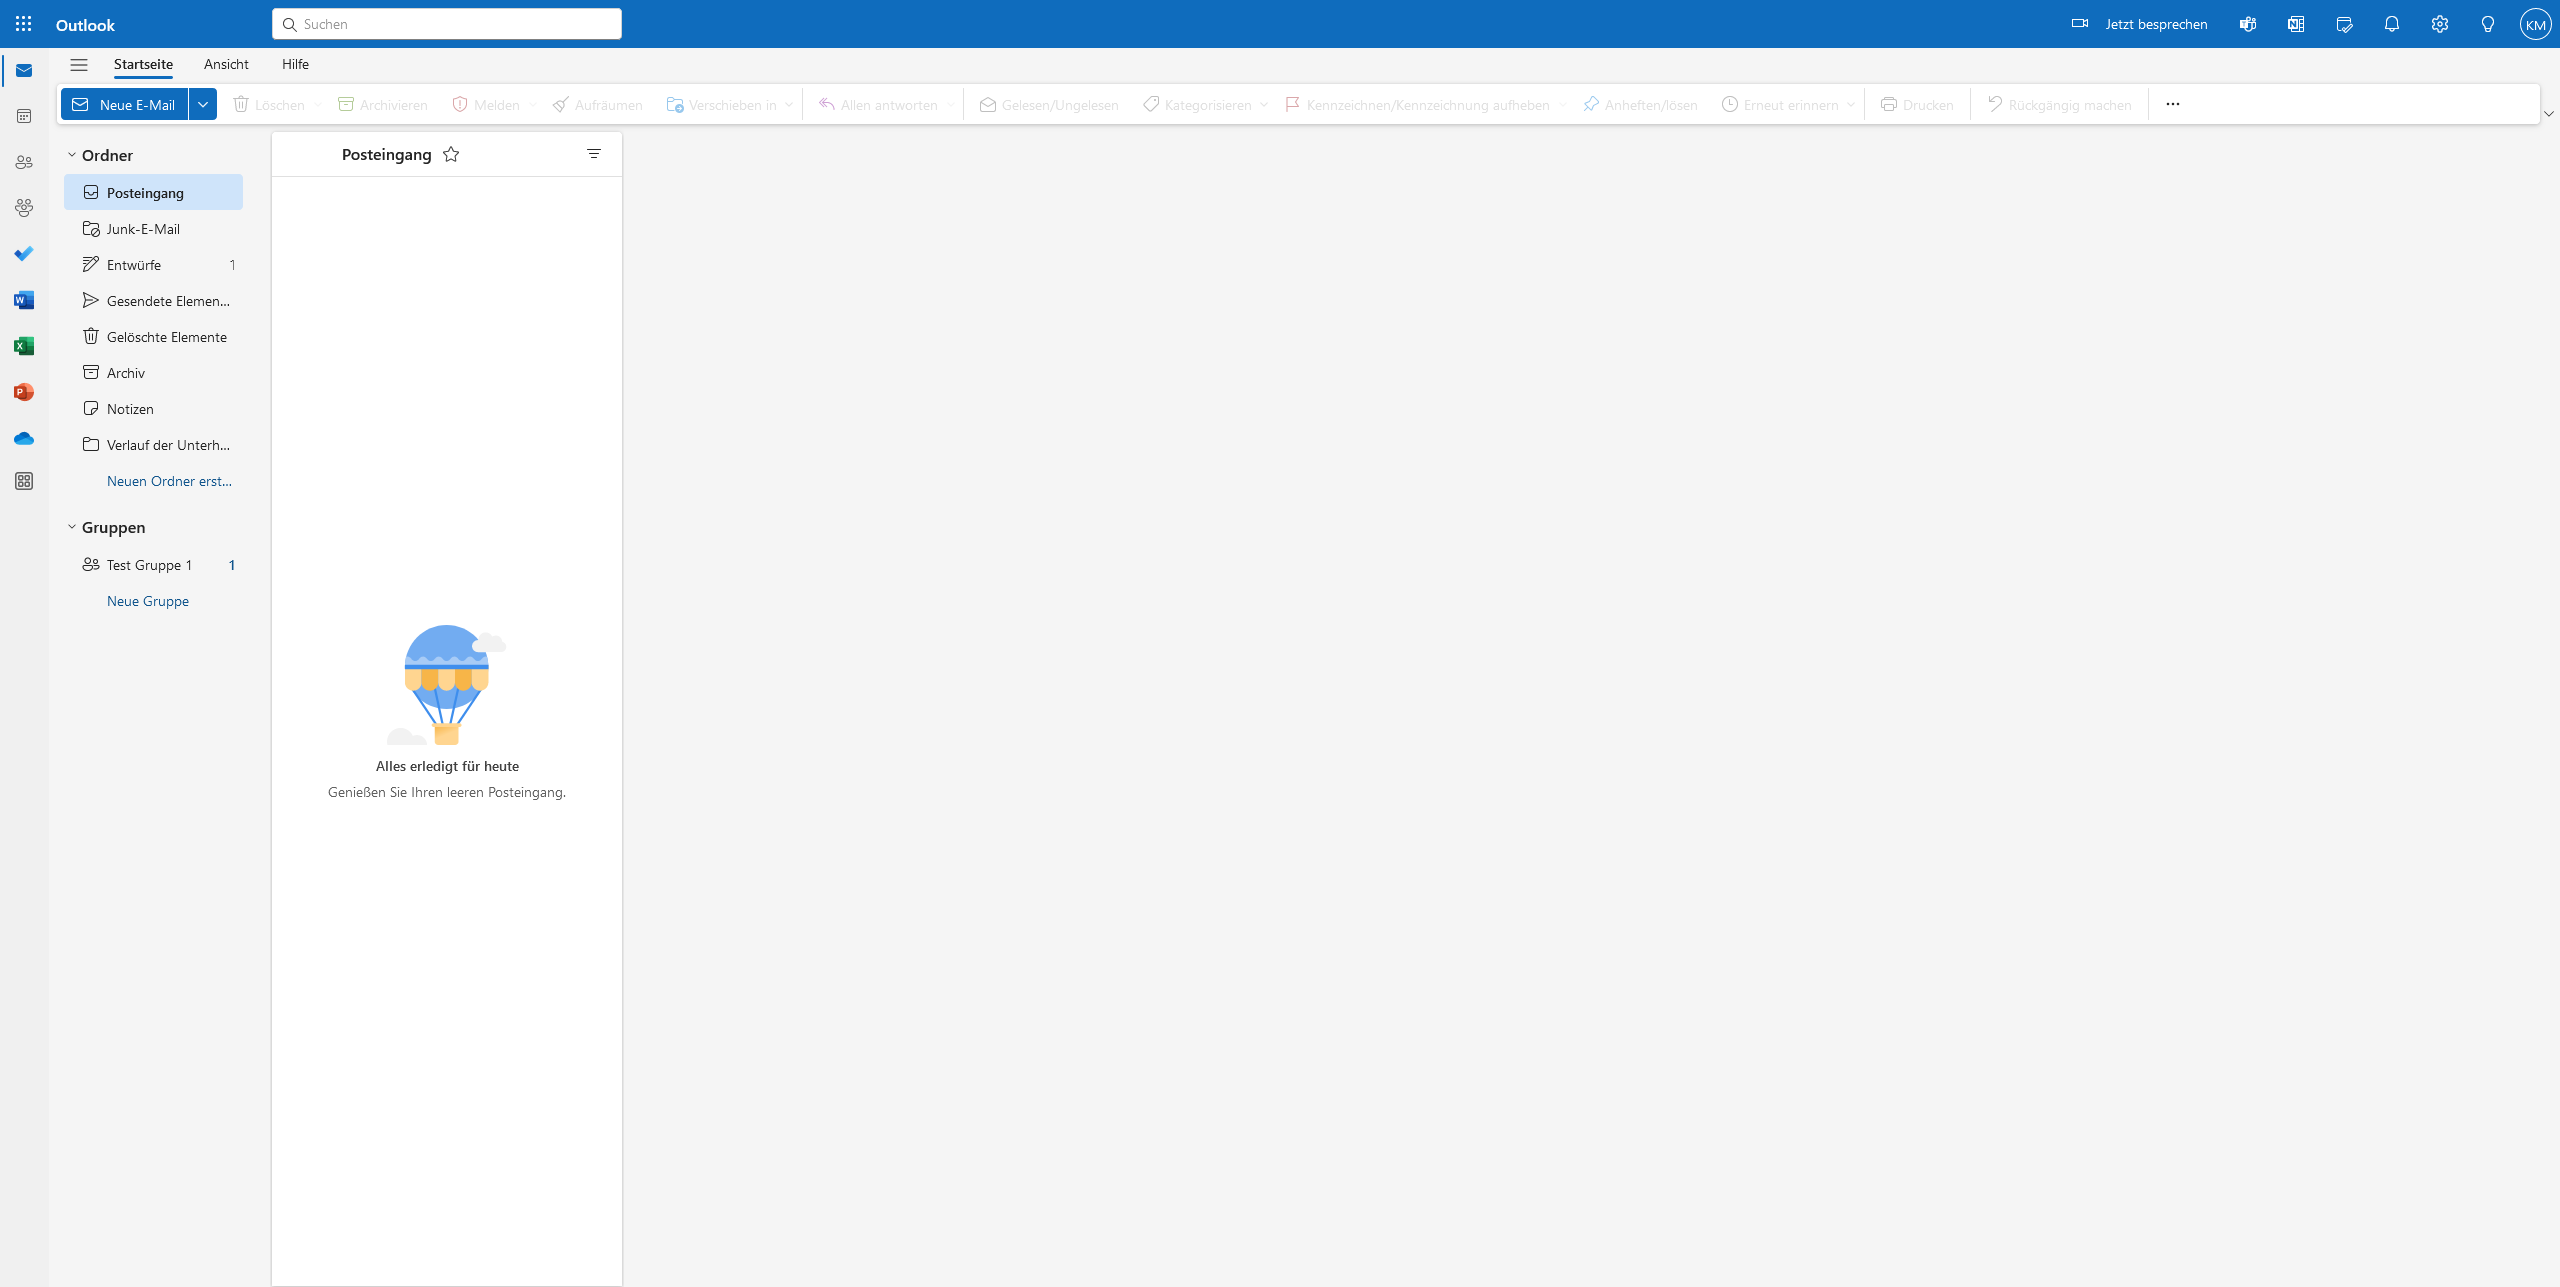
\includegraphics[width=0.75\textwidth]{images/OutlookLive_Mail1.png}
    \caption{OutlookLive Mail}
    \label{fig:outlook-live-mail}
\end{figure}

Die erste Hauptfunktion die Groupwaresysteme erfüllen ist das anbieten eines E-Mail Clients  über den E-Mails empfangen, versendet und verwaltet werden können.
Dabei sollten sich auch mehrere E-Mail Postfächer gleichzeitig hinzugefügt werden können.


\begin{figure}[H]
    \centering
    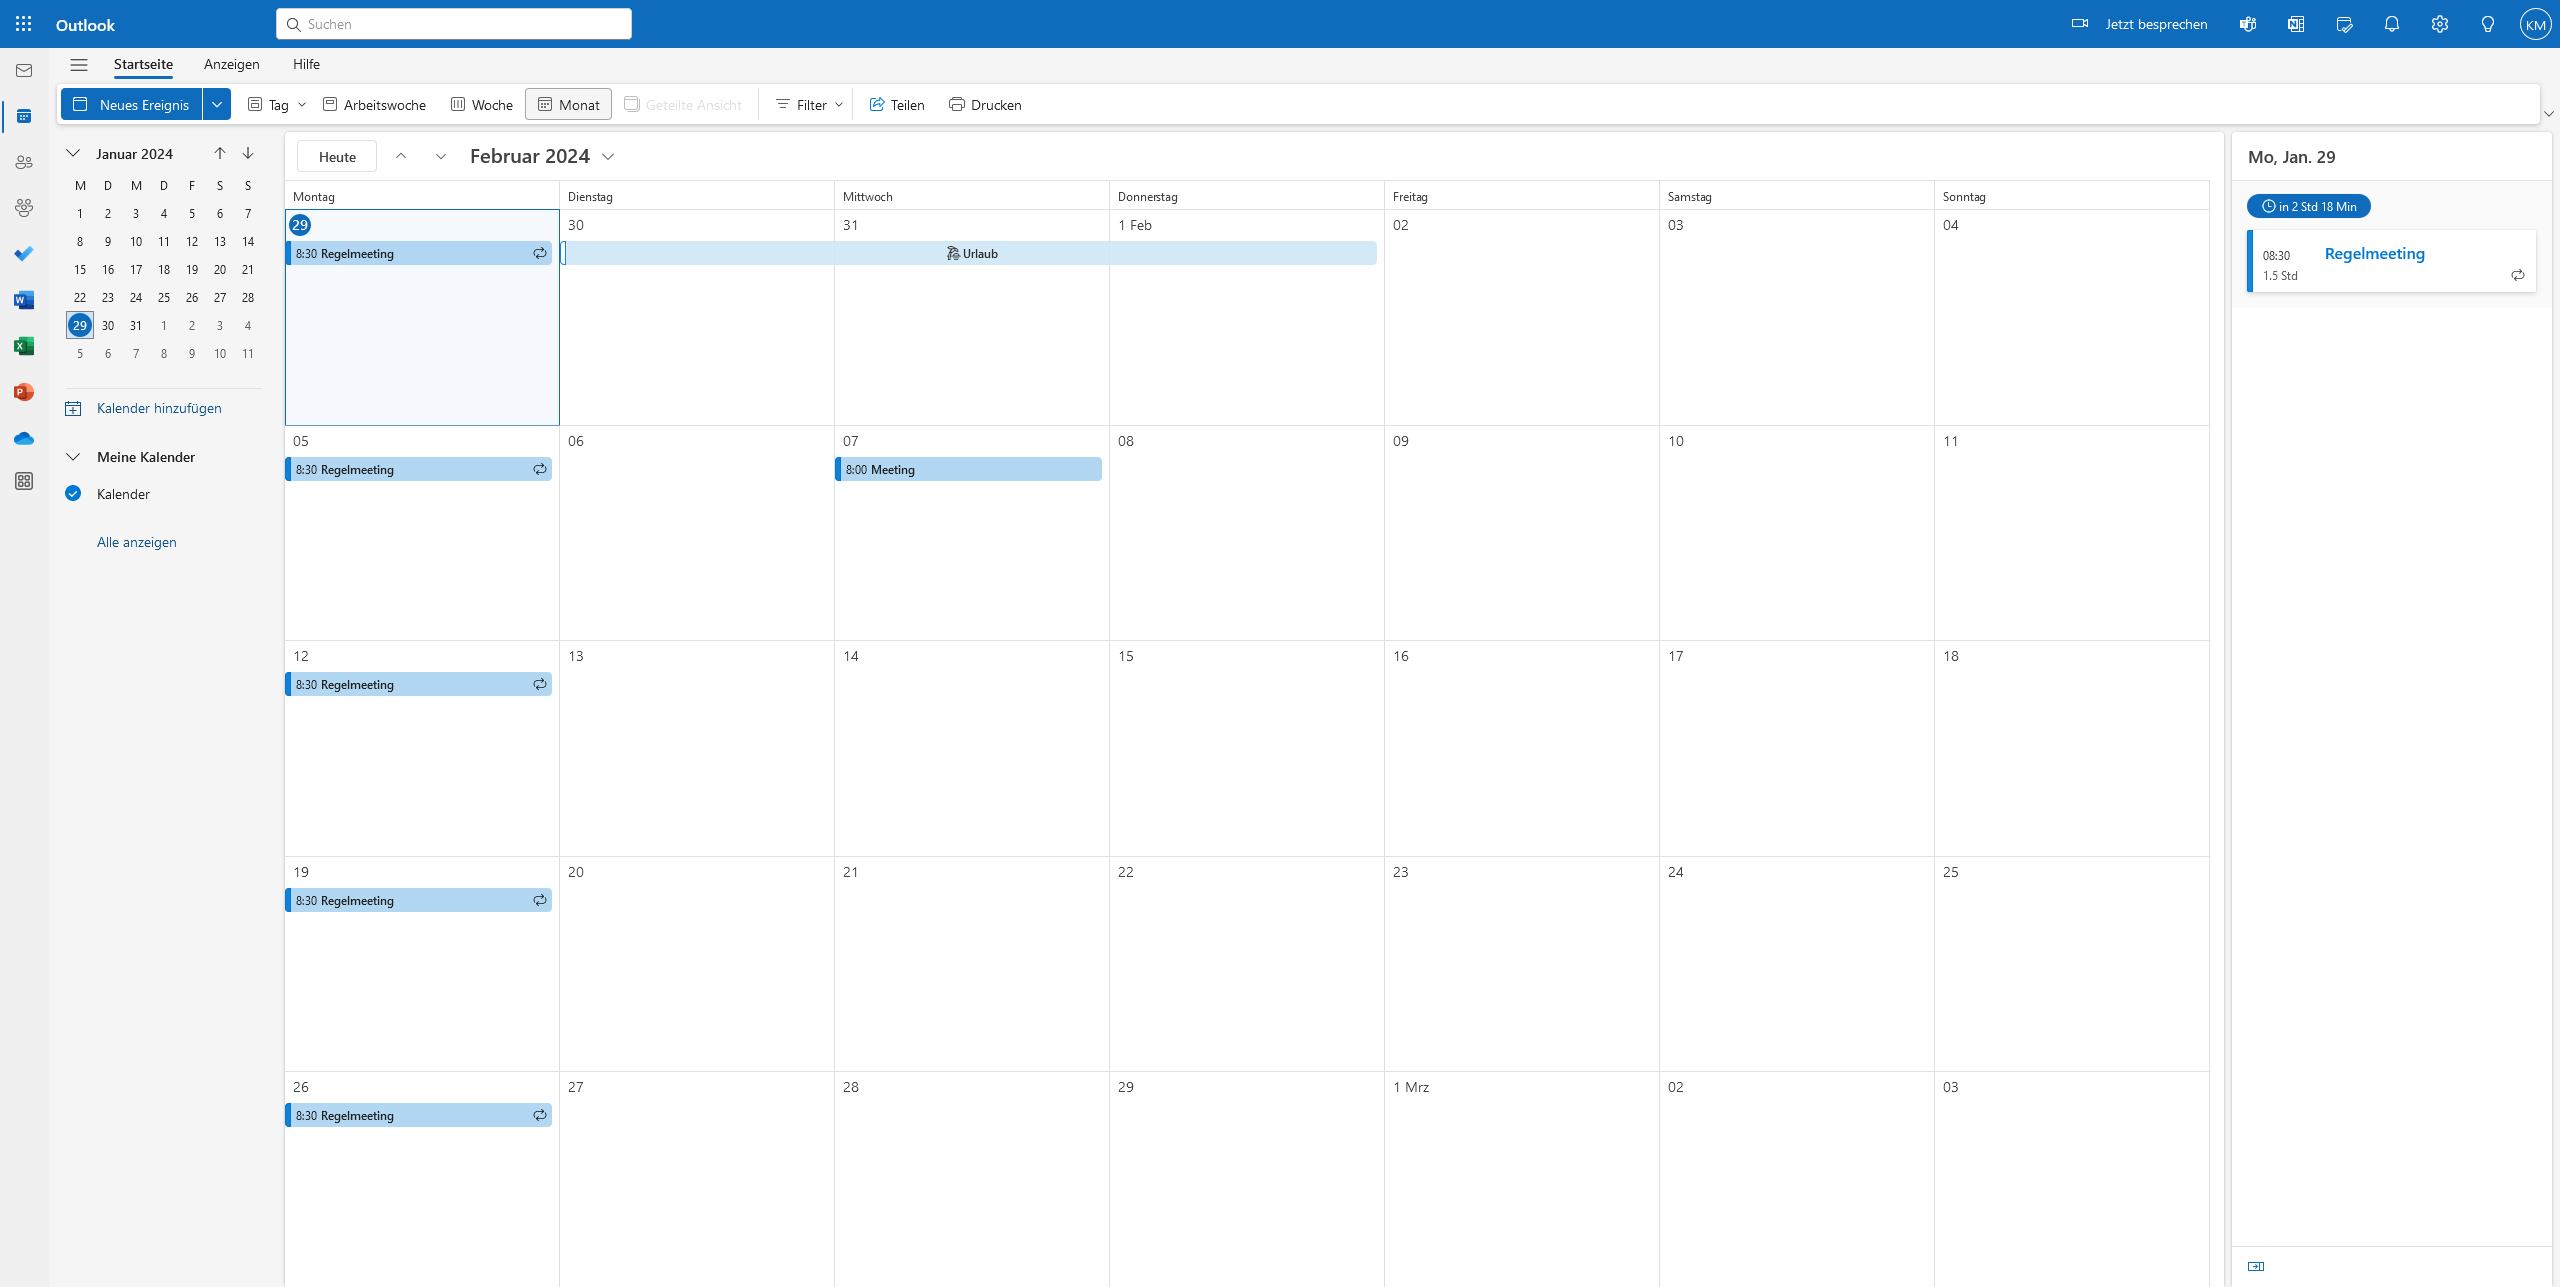
\includegraphics[width=0.75\textwidth]{images/OutlookLive_Calender1.png}
    \caption{OutlookLive Calender}
    \label{fig:outlook-live-calender}
\end{figure}

Eine weitere Hauptfunktion von Groupwaresystemen ist der Kalender, mit dem Terminplanung ermöglicht wird.
Die Terminplanung sollte zudem das Einladen von anderen Nutzern ermöglichen um die Zusammenarbeit und Organisation der Nutzer miteinander zu vereinfachen.
Dabei sollten auch Regeltermine, also Termine die sich regelmäßig wiederholen erstellt werden können.

\begin{figure}[H]
    \centering
    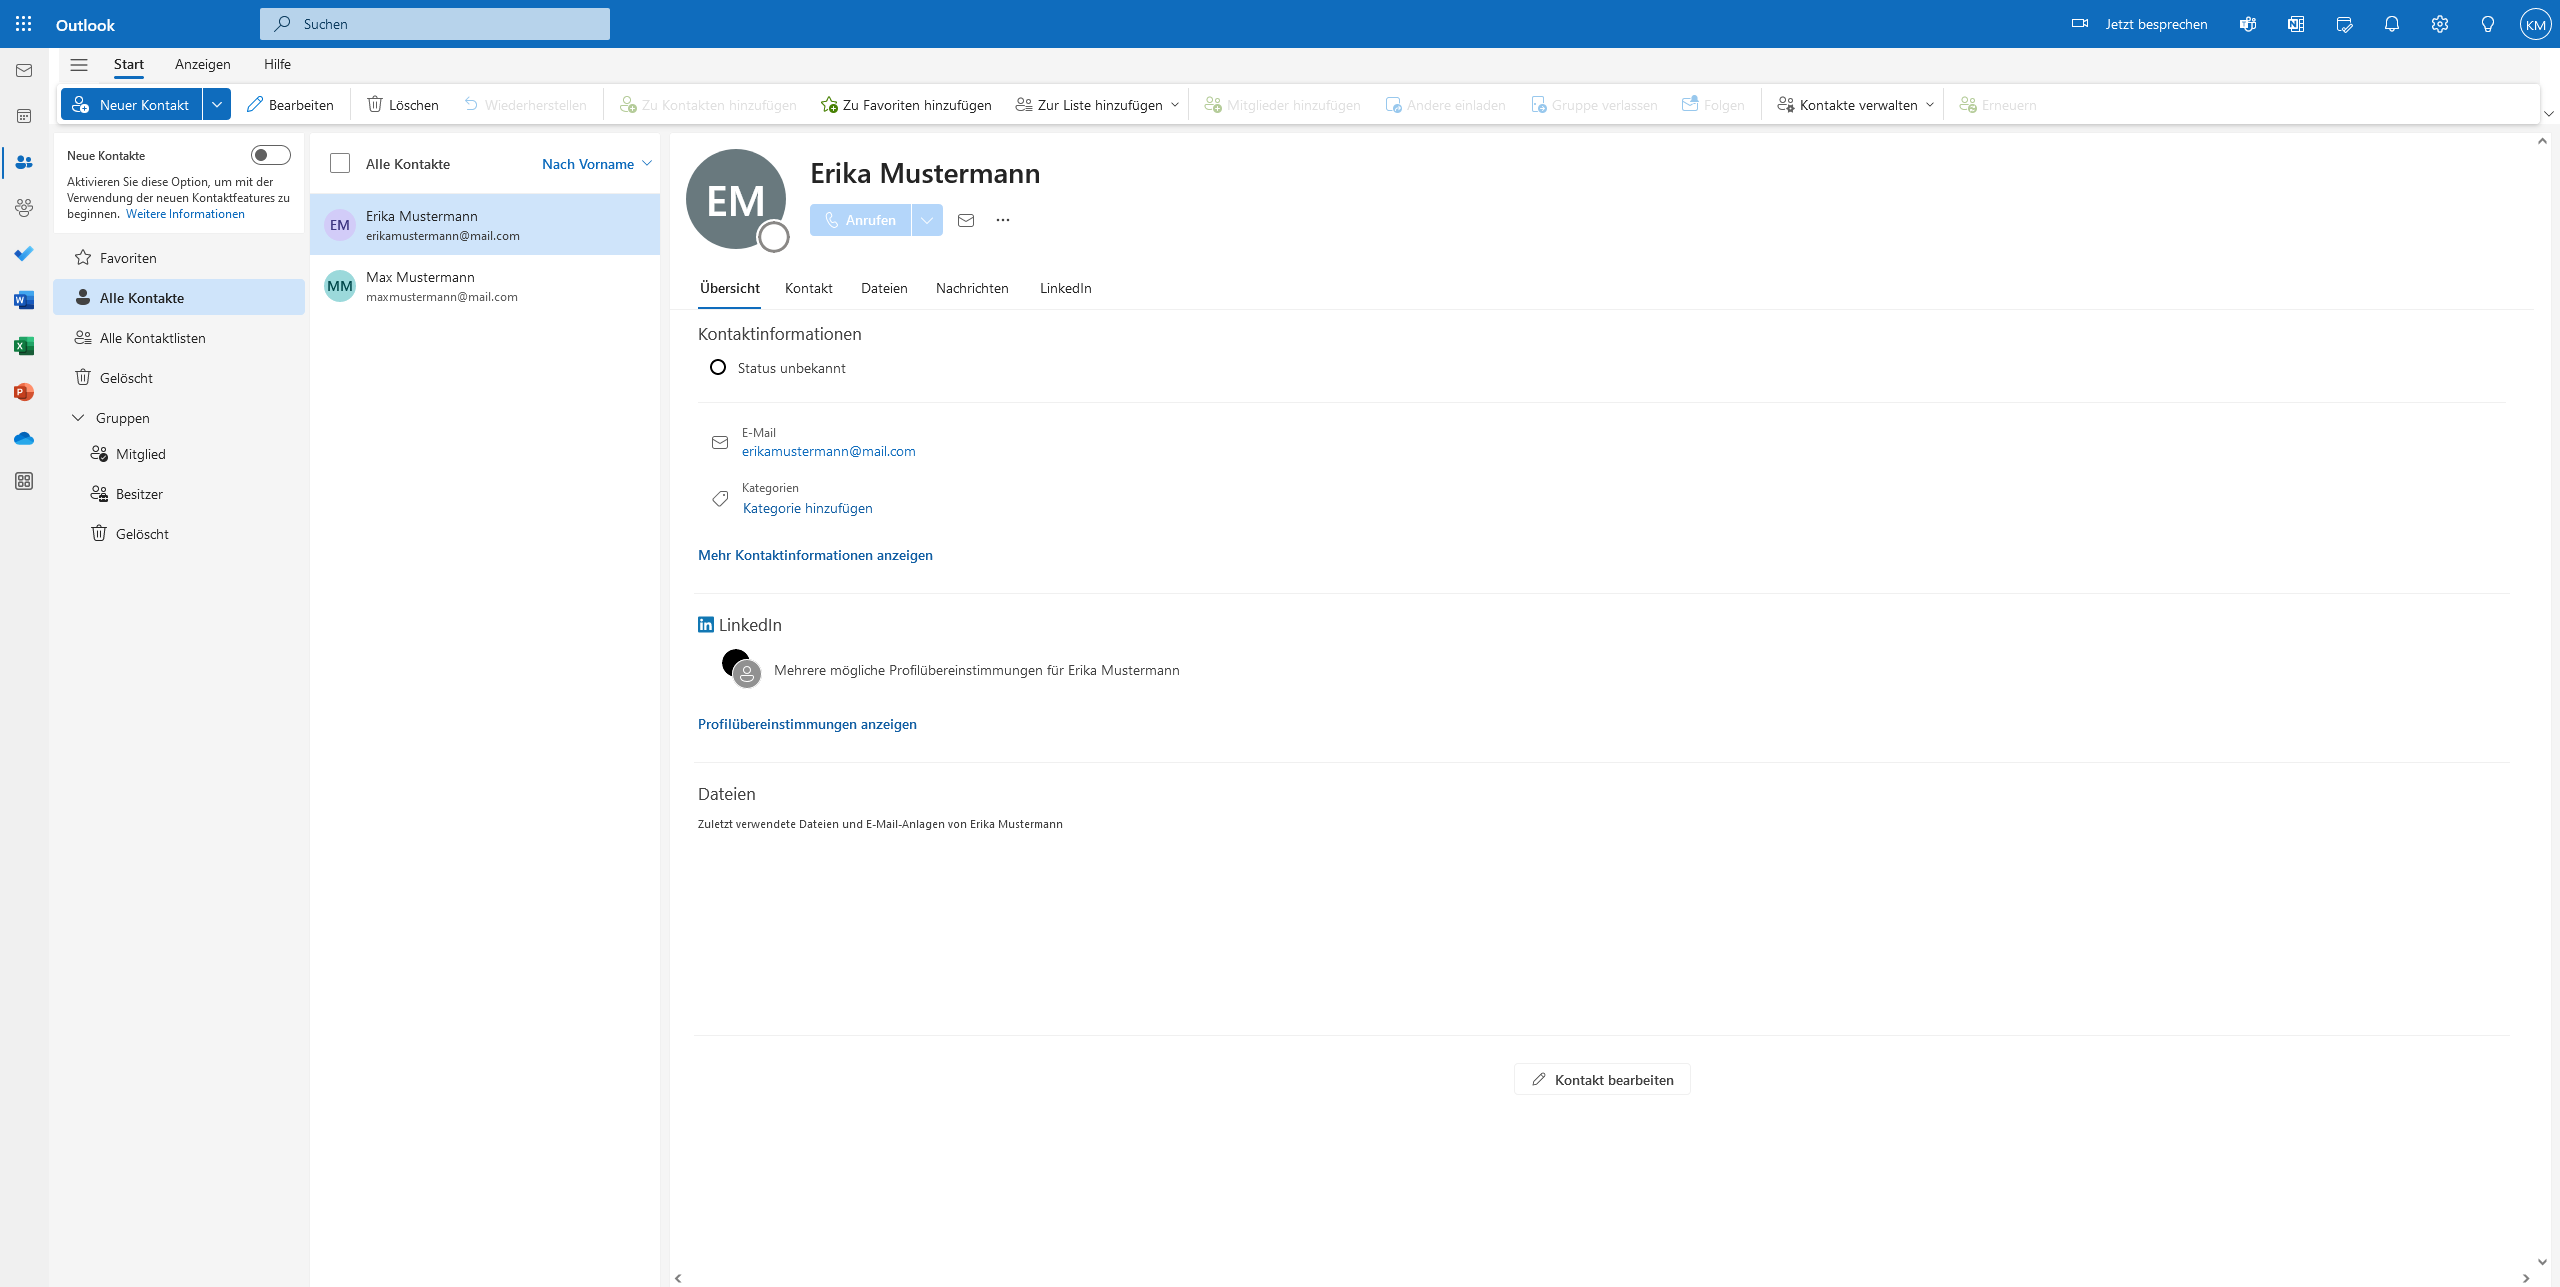
\includegraphics[width=0.75\textwidth]{images/OutlookLive_Contacts.png}
    \caption{OutlookLive Contacts}
    \label{fig:outlook-live-contacts}
\end{figure}

Kontakte sind eine esentieller Bestandteil von Groupwaresystemen um die Vernetzung innerhalb von Arbeitsgruppen zu organisieren.
Durch sie sollte die Kontaktaufnahme zu anderen Gruppenmitgliedern so einfach wie möglich gestaltet werden.
Im Beispiel von OutlookLive kann man beispielsweise wie in Abbildung \ref{fig:outlook-live-contacts} direkt vom Kontakt einer Person diese Person kontaktieren.


\section{Playwright}

Die Open-Source-Bibliothek Playwright wurde Anfang 2020 von Microsoft veröffentlicht und ermöglicht es, Browser automatisiert zu steuern und dadurch automatisierte Tests für Webanwendungen durchzuführen oder Websites zu scrapen.
Dabei bietet Playwright ein Application-Programming-Interface (API) für die Programmiersprachen JavaScript, TypeScript, Python, .NET und Java sowie eine Vielzahl von Funktionen, die das Testen von Webanwendungen erleichtern.
Beispielsweise kann mit Playwright Codegen die eigene Interaktion mit einer Webanwendung augezeichnet und als Code exportiert werden, der dann als Test für die ausgeführte Interaktion verwendet werden kann.
So können effizient Frontend-Tests für eine Vielzahl von Anwendungen implementiert werden.
\autocite[Quelle:][]{playwright}

Im Fall der Studienarbeit wurde Playwright verwendet, um automatisierte Tests für eine der recherchierten Groupware-Systeme durchzuführen.
Dabei werden Frontend-Tests implementiert, die typische Interaktionen mit der Benutzeroberfläche simulieren.
So können beispielsweise Formulare ausgefüllt oder Buttons angeklickt werden, womit ein Nutze-Login und das anschließende aufrufen der Mails des Nutzers simuliert werden kann.

Deckt man mit diesen Tests alle Funktionsbereiche des Groupwaresystems ab, kann man durch das Ausführen der Tests sicherstellen, dass die Anwendung nach einer Änderung noch wie erwartet funktioniert.
Auch falls die Anwendung in Zukunft unerwartete Ausfälle generiert, können diese durch die Tests schneller genauer erkannnt werden.
Geht beispielsweise der zuvor erwähnte Test des aufrufen der Mails schief, gibt es mit hoher Wahrscheinlichkeit ein Problem mit der Verbindung zum Mail Server.







\chapter{Technologien} % DeepL korrigiert

In diesem Kapitel wird ein Überblick über die Technologien gegeben, die zum Implementieren der Prototypen zu den Interaktionskonzepten genutzt werden.
Im Folgenden wird zunächst auf die Hardware eingegangen, wobei das verwendete Anzeigegerät für AR, die Meta Quest 3, näher erläutert wird.
Im Anschluss erfolgt eine Vorstellung der Software-Frameworks, in welchen die Prototypen implementiert werden.

\section{Meta Quest 3}

Im Rahmen der Bachelorarbeit wird als Anzeigegerät für die AR-Anwendung die Meta Quest 3 verwendet.
Hierbei handelt es sich um ein Standalone-AR- und VR-Headset, welches von Meta (ehemals Facebook) entwickelt wurde und Ende 2023 auf den Markt kam.
Das HMD ist mit einem eigens für mobile XR-Geräte entwickelten Qualcomm Snapdragon XR2 Gen2 Prozessor ausgestattet, wodurch es selbst in der Lage ist, anspruchsvolle Inhalte zu rendern.
Es muss nicht wie viele andere HMDs an einen Computer oder ein Smartphone angeschlossen werden, sondern kann direkt allein verwendet werden.
Das Headset verfügt beispielsweise auch über einen eigenen Browser, wodurch AR-Anwendungen auch einfach übers Internet aufgerufen werden können.
Dieses Nutzen von Anwendungen über den Browser wird auch für die Prototypen dieser Arbeit genutzt, worauf in Kapitel \ref{section:webxr} genauer eingegangen wird.

Das Headset verfügt über zwei Displays mit einer Auflösung von jeweils 2064 x 2208 Pixeln und einer Bildwiederholrate von bis zu 120 Hz.
Dadurch werden Inhalte mit einer hohen Bildqualität und einer flüssigen Darstellung angezeigt.
Die Kombination der geringen Latenz aufgrund des On-Board-Prozessors mit der hohen Bildwiederholrate resultiert in einer hohen Immersion und einem angenehmen Nutzungserlebnis.

\newpage

Darüber hinaus verfügt die Meta Quest 3, wie in Abbildung \ref{fig:quest-front-cameras} dargestellt, über zwei RGB-Kameras (untere Kameras), zwei IR-Kameras (obere Kameras) sowie einen Tiefenprojektor (schwarze Fläche in der Mitte) auf der Vorderseite, welche gemeinsam die Umgebung des Nutzers erfassen und so AR-Anwendungen mittels Image-Passthrough ermöglichen.

\begin{figure}[H]
  \centering
  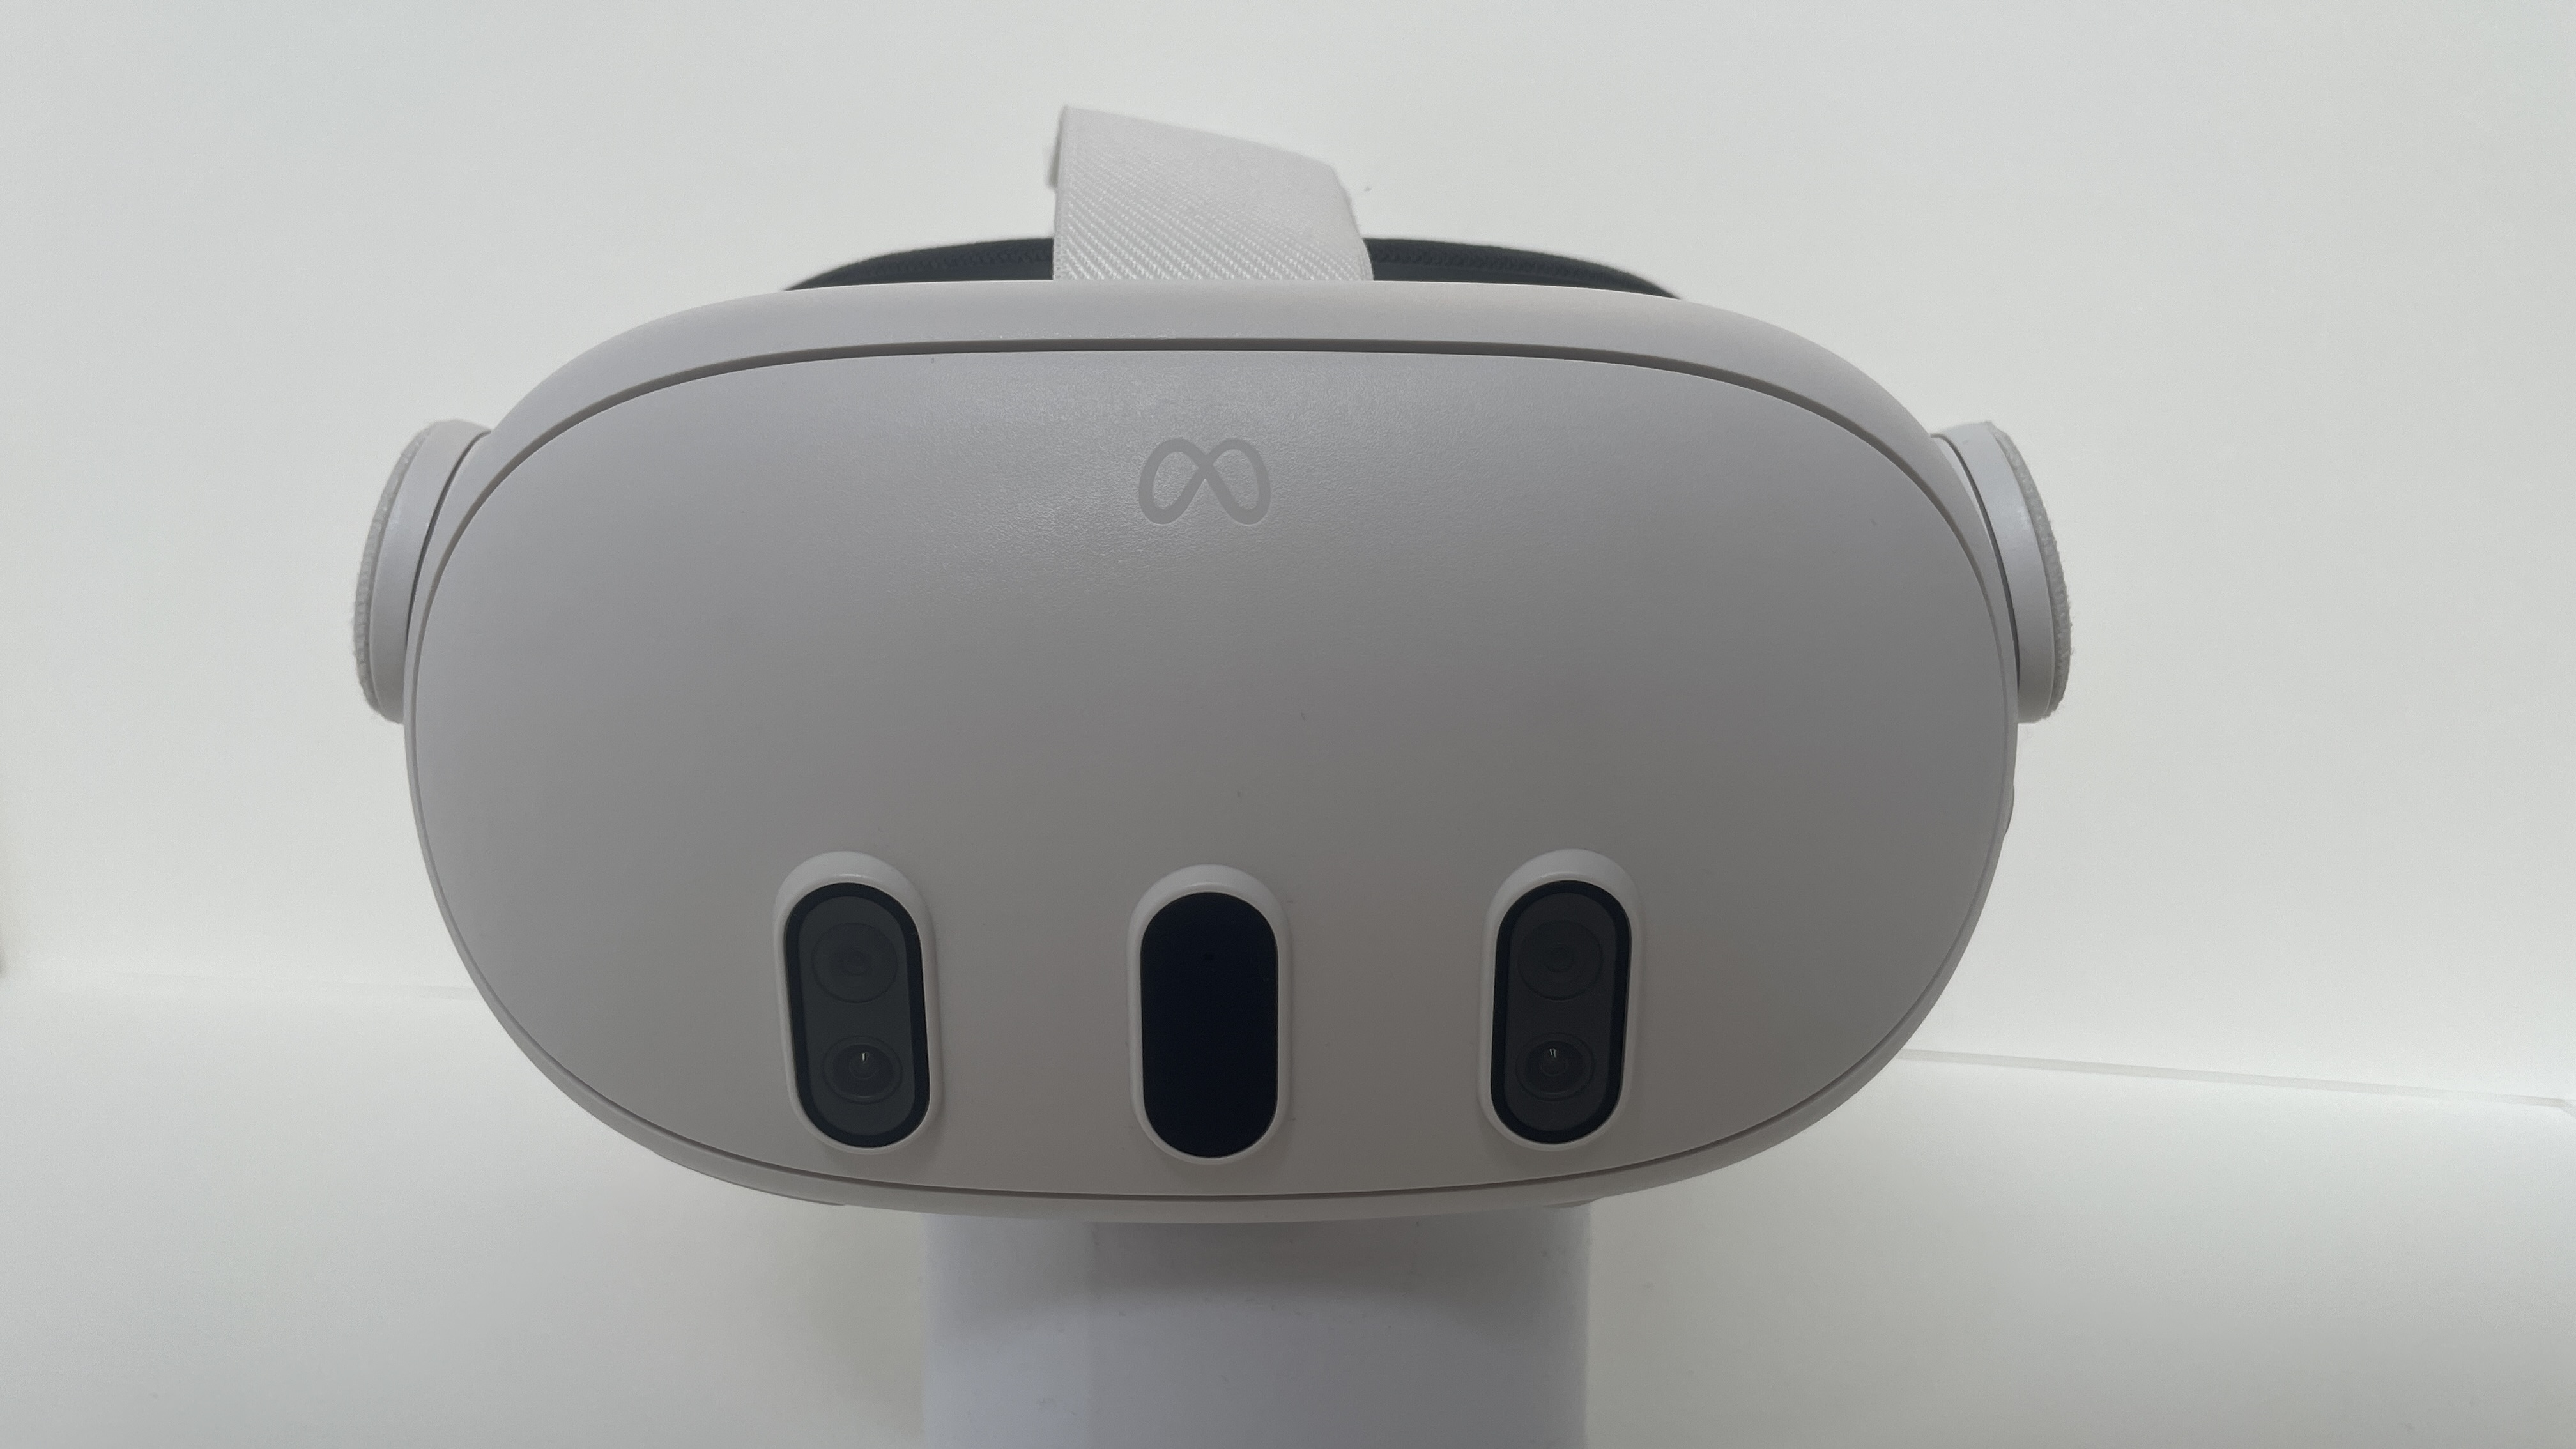
\includegraphics[width=0.7\textwidth]{images/Oculus-FrontCameras.jpg}
  \caption{Frontal ausgerichtete Kameras und Tiefenprojektor der Meta Quest 3}
  \label{fig:quest-front-cameras}
\end{figure}

Zusätzlich zu den zwei RGB-Kameras sind insgesamt noch vier Infrarot-Kameras auf dem Headset verbaut, zwei davon auf der Vorderseite, direkt über den RGB-Kameras, und zwei auf der Unterseite.
Über diese Kameras wird die Position des Nutzers im Raum kontinuierlich getrackt und angepasst, sodass auf externe Trackingstationen verzichtet werden kann.

Die Meta Quest ermöglicht zudem die Erkennung und das Tracking der Hände des Nutzers mithilfe der vier Infrarotkameras und zwei RGB-Kameras als alternative Eingabegeräte.
Dadurch kann der Nutzer seine eigenen Hände in VR- und AR-Anwendungen als Eingabegerät verwenden. \autocite[]{meta-quest-3}.
Dafür sind auch zwei der vier Infrarotkameras wie in Abbildung \ref{fig:quest-hand-cameras} zu sehen ist nach unten gerichtet, um die Hände des Nutzers jederzeit tracken zu können.

\begin{figure}[H]
  \centering
  \includegraphics[width=1\textwidth]{images/Oculus_DownCameras.png}
  \caption{Die beiden nach unten gerichteten Kameras der Meta Quest 3}
  \label{fig:quest-hand-cameras}
\end{figure}


\section{WebGL}

WebGL ist eine JavaScript-API, die das Rendern von 3D-Grafiken in einem Webbrowser ermöglicht.
Die WebGL-Spezifikation wird von der Khronos Group entwickelt, einer Non-Profit-Organisation, welche als ein Zusammenschluss aus über 180 Unternehmen aus der Tech-Industrie technologische Standards entwickelt.
Zu den Unternehmen, die an der Entwicklung von WebGL beteiligt sind, gehören auch die Unternehmen, die die größten Browser der Industrie entwickeln: Google (Chrome), Mozilla (Firefox), Apple (Safari) und Microsoft (Edge) \autocite[]{khronos-webgl, khronos-about}.
Aufgrund dieser Mitarbeit verschiedener Unternehmen und der offenen Entwicklung der Spezifikation kann WebGL in fast allen modernen Webbrowsern verwendet werden.

WebGL basiert dabei auf der OpenGL ES Spezifikation, welche, ebenfalls von der Khronos Group, speziell für Embedded Systems und mobile Systeme, also zum Großteil Systeme ohne eigene Grafikkarte, entwickelt wurde \autocite[]{khronos-opengles}.
Aufgrund dieser Ausrichtung auf mobile Geräte, können mit WebGL Anwendungen entwickelt werden, die auf einfachen Geräten wie Smartphones oder aber auch auf VR- und AR-Headsets ohne zusätzliche Rechenleistung laufen \autocite[][S.3]{Baruah2021}.


\section{WebXR}
\label{section:webxr}

Die WebXR-API ist eine standardisierte Schnittstelle für Webanwendungen, die die Erstellung immersiver VR- und AR-Anwendungen für das Internet ermöglicht.
Das World Wide Web Consortium (W3C), welches die WebXR-Standards definiert beschreibt WebXR wie folgt: \glqq{}Die WebXR Device API bietet die notwendigen Schnittstellen, damit Entwickler ansprechende, komfortable und sichere immersive Anwendungen im Web für eine Vielzahl von Hardware-Formfaktoren erstellen können\grqq{} \autocite[aus dem Englischen mit DeepL ][1. Introduction]{w3c_webxr}.
Mit WebXR entwickelte Anwendungen können als Webanwendungen direkt von einem Webbrowser eines AR- oder VR-Geräts aus aufgerufen werden, ohne dass eine zusätzliche Installation der Anwendung notwendig ist.

Der Ablauf von WebXR-Anwendungen ist in Abbildung \ref{fig:webxr-app-flow} dargestellt.
Dabei wird zuerst beim Aufrufen der Anwendung geprüft, ob die angegebene Art von XR-Inhalt von der Hardware und dem User Agent (UA) unterstützt werden.
Der User Agent der Software bezeichnet dabei die Software, mit welcher der Nutzer auf die Anwendung zugreift, also den Webbrowser des Nutzers. 
Ist die Art des XR-Inhalts von der Technik des Nutzers unterstützt, kann die XR-Session vom Nutzer manuell über einen Knopf gestartet werden.
Nach erfolgreichem Start der Session wird der Frame Loop der Anwendung gestartet.
Der Frame Loop ist eine Schleifenfunktion, die kontinuierlich während der XR-Session ausgeführt wird um die einzelnen Frames, bzw. Bilder, für das XR-Display zu rendern.
Dieser Frame Loop läuft, bis die Session durch den UA beendet wird.
Befindet sich der UA noch auf der Seite der WebXR-Anwendung, wird wieder der Knopf zum Starten der XR-Session angezeigt, falls der Nutzer direkt wieder eine neue Session starten möchte.

\begin{figure}[H]
    \centering
    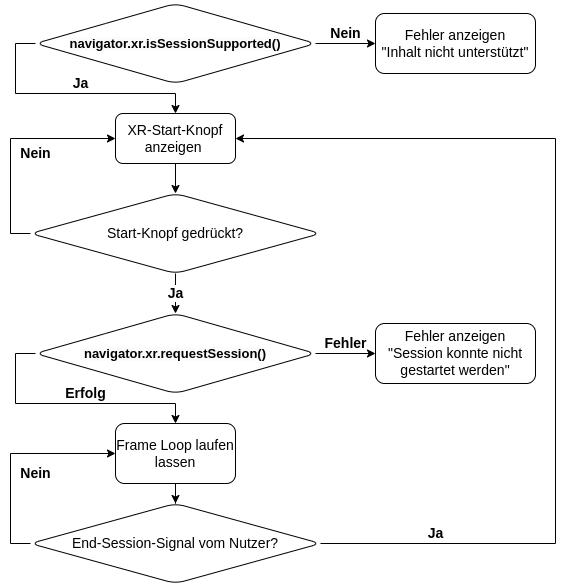
\includegraphics[width=0.6\textwidth]{images/WebXR-App-Flow.png}
    \caption{Application Flow von WebXR-Anwendungen}
    \source{nach \autocite[][Kap. 1.2. Application Flow]{w3c_webxr}}
    \label{fig:webxr-app-flow}
\end{figure}

\subsubsection{Three.js}

Three.js ist eine Open-Source-JavaScript-Bibliothek, die unter der MIT-Lizenz steht und auf WebGL basiert.
Sie vereinfacht die Erstellung und Darstellung von 3D-Grafiken in Webanwendungen.
Die Bibliothek bietet eine Vielzahl von Funktionen, die es Entwicklern ermöglichen, detaillierte 3D-Modelle und -Szenen zu erstellen und zu rendern \autocite[][]{threejs-docs}.
Dabei unterstützt Three.js auch die Erstellung von AR- und VR-Anwendungen mithilfe von WebXR.

Des Weiteren existieren Frameworks, die auf der Three.js API basieren und die Entwicklung von AR- und VR-Anwendungen sowie 3D-Anwendungen im Allgemeinen weiter vereinfachen. 
Ein Beispiel dafür ist das Framework A-Frame, welches auf die Entwicklung von AR- und VR-Anwendungen spezialisiert ist und Funktionen einer nahezu vollwertigen Game-Engine bietet \autocite[]{a-frame-introduction}.

Zudem wird Three.js von vielen Entwicklern und Unternehmen verwendet und hat dadurch eine große Community und viele Ressourcen und Tutorials, welche Entwicklern bei der Erstellung und Fehlerbehebung ihrer Anwendungen behilflich sein können.

Die Vielzahl an Funktionen sowie die große Nutzerbasis machen Three.js, insbesondere in Kombination mit A-Frame, zu einer vielversprechenden Option für die Entwicklung von AR- und VR-Anwendungen.
Jedoch ergaben sich in den ersten Tests der Funktionalität von Three.js und A-Frame im Browser der Meta Quest 3 Probleme mit der Erkennung der AR-Brille und der Darstellung von AR-Inhalten.

\subsubsection{Babylon.js}

Babylon.js ist eine Open-Source-Rendering- und Game-Engine, die in einer JavaScript-Bibliothek verpackt ist.
Sie wird unter anderem von einem Team von Entwicklern bei Microsoft entwickelt.
Die Bibliothek bietet Support für WebGL 1.0/2.0 sowie WebGPU und verfügt über eine Vielzahl von Funktionen, die es Entwicklern ermöglichen, detaillierte 3D-Modelle und -Szenen zu erstellen und zu rendern.
Darüber hinaus bietet es native Unterstützung sowie eine Dokumentation für WebXR, wodurch die Entwicklung von VR- und AR-Anwendungen vereinfacht wird \autocite[][]{babylon-features}.

Die Bibliothek bietet dabei auch viele Quality-of-Life-Features, wie beispielsweise einen Szenen-Explorer und -Inspektor, der sich für die Entwicklung und das Debugging von 3D-Szenen direkt im Browser eignet und mit einer Zeile Code in die Anwendung eingebunden werden kann.
Über den Szenen-Explorer, welcher in Abbildung \ref{fig:babylon-inspector} links dargestellt ist, können aus dem Szenengraph der aktuellen Szene Objekte ausgewählt werden um im Szenen-Inspektor eine Detailansicht des Objekts und seinen Eigenschaften zu erhalten.
Mithilfe des Szenen-Inspektors, welcher in Abbildung \ref{fig:babylon-inspector} rechts dargestellt ist, können dann in Echtzeit die Eigenschaften von Objekten betrachtet und verändert werden.

\begin{figure}[H]
  \centering
  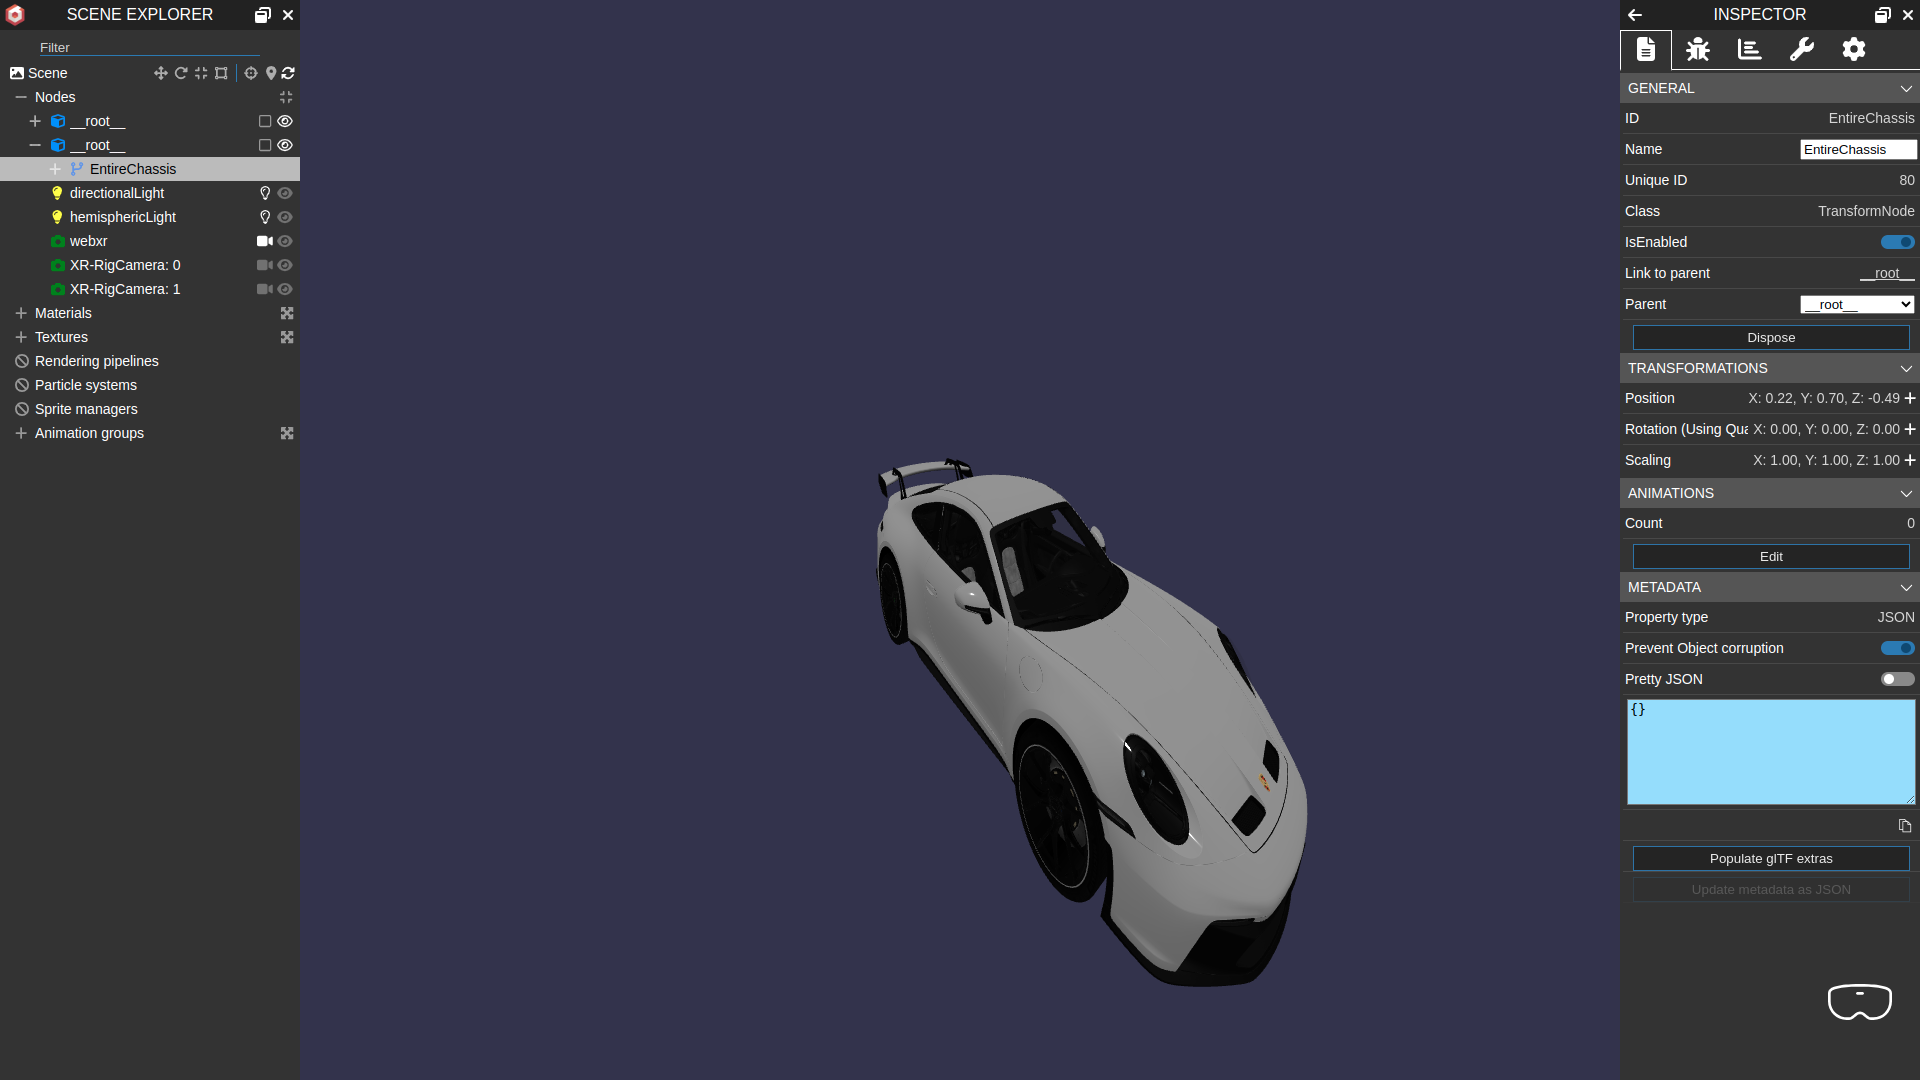
\includegraphics[width=1\textwidth]{images/BabylonInspector.png}
  \caption{Szenen-Explorer und -Inspektor von Babylon.js}
  \label{fig:babylon-inspector}
\end{figure}

% 1x Durchgelesen (02.07)

%DeepL korrigiert
\chapter{Konzept}
\label{section:konzept}

Die vorliegende Bachelorarbeit beschäftigt sich mit der Darstellung von Requirements in Augmented Reality.
Im Rahmen dessen wird untersucht, wie Requirements in einer 3D-Umgebung dargestellt werden könnten.
Dazu werden verschiedene Interaktionskonzepte entwickelt, welche als Basis für die Implementierung von Prototypen mit WebXR dienen.
Die erste Ausarbeitung der Konzepte dient dabei nicht unbedingt dazu, vollständig so implementiert zu werden, sondern soll einen Überblick über die grundlegende Idee und die möglichen Interaktionen geben.

%DeepL korrigiert

\section{Explodierende Bauteile}

Das erste untersuchte Interaktionskonzept ist hauptsächlich für die Darstellung von Requirements von physischen Produkten gedacht.
Die Idee ist, ein Produkt in einer Animation in seine einzelnen Bauteile zu zerlegen und die Requirements direkt an ihren zugehörigen Bauteilen darzustellen.
In der Animation werden die Bauteile wie in der Bildsequenz in Abbildung \ref{fig:rubiks-explosion} von einem Punkt in der Mitte des Produkts nach außen bewegt, sodass sie sich um den Ursprungspunkt des Produkts herum anordnen.
Ein Fahrzeug könnte beispielsweise so zerlegt werden, dass sich bei der Animation die Räder, die Karosserie, der Motor und die Innenausstattung einzeln als eigene Objekte auseinanderbewegen.
Auf diese Weise kann der Nutzer das gesamte Produkt betrachten und sich dann auf Wunsch einzelne Bauteile und deren Requirements genauer ansehen. 
Im Beispiel des Rubiks Cube aus Abbildung \ref{fig:rubiks-explosion} wäre dann jeder Würfel ein Bauteil, der seine eigenen Requirements angehängt bekommen würde.


%DeepL korrigiert

\begin{figure}[H]
    \centering
    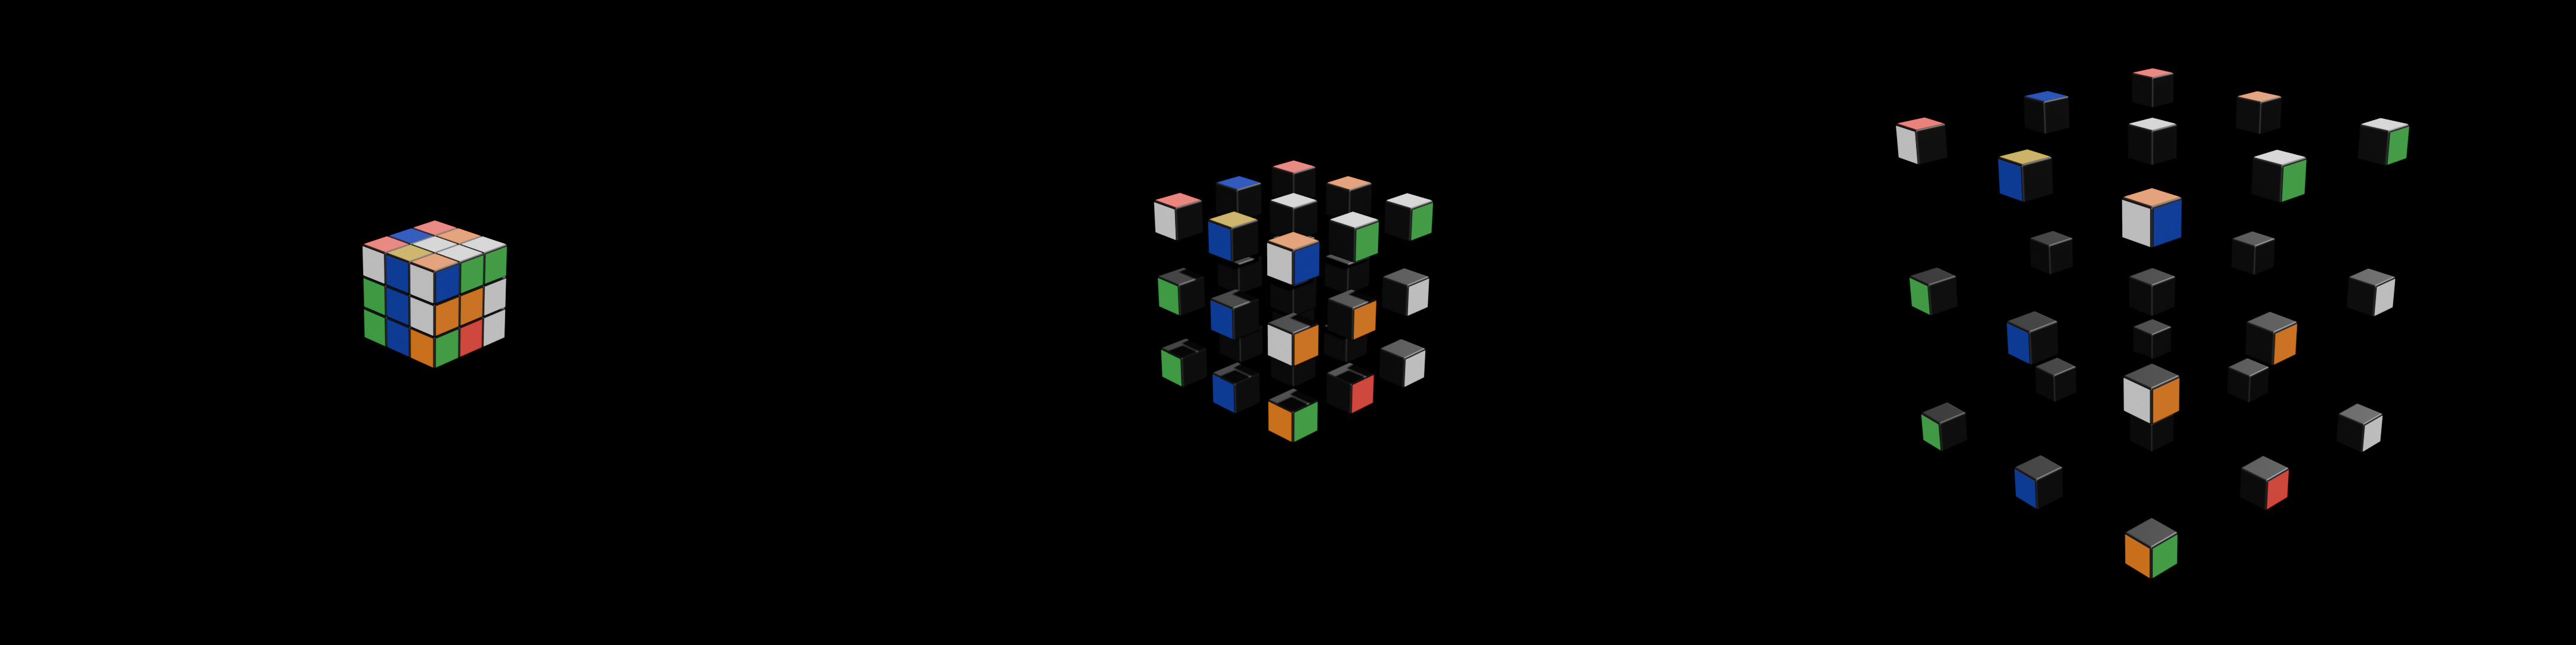
\includegraphics[width=1\textwidth]{images/RubiksExplosion.png}
    \caption{Beispiel einer Explosionsanimation anhand eines Rubiks Cube}
    \label{fig:rubiks-explosion}
\end{figure}

Die Requirements sollen in Form von Text auf UI-Panels dargestellt werden, welche an den zugehörigen Bauteilen angebracht sind.


Bei komplexen Produkten mit einer Vielzahl an Bauteilen, wie beispielsweise einem Fahrzeug, existiert eine hohe Anzahl an Requirements.
Eine gleichzeitige Animation aller Komponenten würde dann bei komplexen Produkten zu einer übermäßigen Zahl an Requirements führen, die gleichzeitig dargestellt werden müssten.
Daher ist es bei umfangreichen Produkten eventuell sinnvoll, die Darstellung der Bauteile in mehreren Schritten zu realisieren.
Dafür könnten Bauteile des Produkts, die aus mehreren anderen Bauteilen bestehen, als separate Produkte mit ihrer eigenen Explosionsanimation betrachtet werden.
Ein Beispiel für eine Komplettübersicht ist die Darstellung eines kompletten Fahrzeugs in wenigen Bauteilen.
Dabei wird ein Rad, das aus Reifen, Felge, Radmuttern, Bremsscheibe etc. besteht, als ein einzelnes zusammengehöriges Objekt behandelt.
Bei Bedarf kann der Nutzer in eine Detailansicht wechseln, in der lediglich ein Rad mit all seinen Bauteilen animiert wird.
Durch eine Verschachtelung von immer detaillierteren Ansichten kann eine hohe Komplexität der Darstellung erreicht werden, ohne dass die Übersichtlichkeit durch eine zu hohe Anzahl an Requirements gleichzeitig verloren geht.
Dieses Prinzip der Verschachtelung ist auch im Ablaufdiagramm in Abbildung \ref{fig:explosions-ablauf} anhand der beiden rechts und links abgehenden Schleifen des unteren Entscheidungsblocks zu erkennen.

\begin{figure}[H]
  \centering
  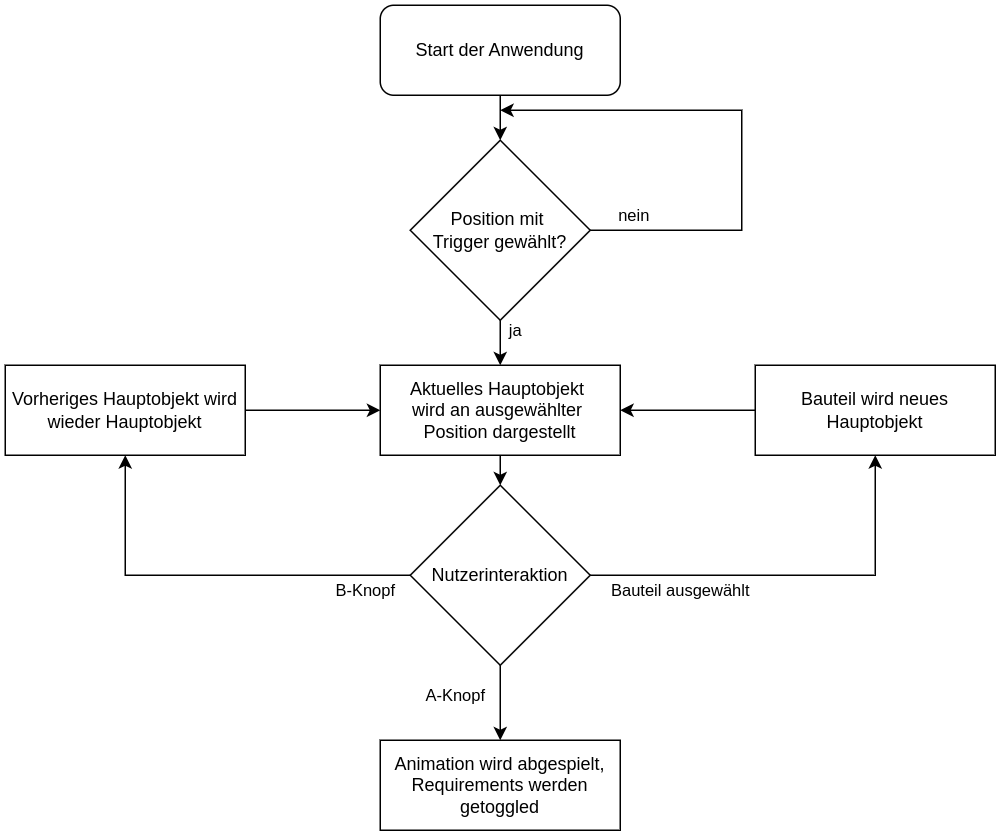
\includegraphics[width=0.8\textwidth]{images/ExplosionAblauf.png}
  \caption{Ablaufdiagramm des Interaktionskonzepts der Explodierenden Bauteile}
  \label{fig:explosions-ablauf}
\end{figure}

Für diese Darstellung soll der Nutzer, wie am ersten Entscheidungsblock im Diagramm in Abbildung \ref{fig:explosions-ablauf} zu sehen ist, zunächst mithilfe eines Controllers einen Ort für die Darstellung im Raum auswählen.
Der ausgewählte Punkt im Raum wird als Ursprungspunkt für die Darstellung der Bauteile verwendet.
Anschließend hat der Nutzer die Möglichkeit, die Explosionsanimation des aktuell angezeigten Modells per Knopfdruck zu aktivieren.
Beim Drücken des A-Knopfs wird dann die Animation des aktuellen 3D-Modells abgespielt und den Bauteilen werden ihre Requirement-Panels angehängt.

Alternativ besteht für den Anwender die Möglichkeit, mit dem Trigger ein anderes Bauteil auszuwählen, um dieses als neues Hauptmodell anzuzeigen und somit dessen Requirements zu betrachten.
Durch Betätigen des B-Knopfes erfolgt eine Reduzierung des Detailgrads der Darstellung, sodass die vorherige Ansicht wiedergegeben wird.

Auch bei Software-Requirements ist es denkbar, diese in ihre Komponenten zu zerlegen und zu diesen Komponenten zugehörige Requirements darzustellen.
Jedoch bietet die Darstellung in AR bzw. VR hierbei quasi keine Vorteile im Gegensatz zu einer 2D-Darstellung auf einem Bildschirm.
Bei Software-Anwendungen ist die einfache Darstellung auf einem Bildschirm näher an der tatsächlichen Laufumgebung der meisten Softwareprodukte weshalb das Konzept eher für physische Produkte sinnvoll ist.

Bereits bei der Erstellung des Konzepts wird ersichtlich, dass einige der Implementierungsschritte, wie beispielsweise das Erstellen der Animation, einen hohen Zeitaufwand erfordern können.
Im Rahmen dieses Interaktionskonzepts soll daher die Realisierbarkeit solcher Darstellungen für physische Produkte untersucht werden.
In diesem Zusammenhang ist zu berücksichtigen, dass aufgrund des zu erwartenden hohen Zeitaufwands für die Implementierung eine kritische Betrachtung der Kosten-Nutzen-Relation erforderlich ist.
Um dennoch eine sinnvolle Grundlage für die tatsächliche Anwendung zu bieten, muss das Interaktionskonzept einen wesentlichen Mehrwert bei der Vermittlung der Requirements aufweisen.
%DeepL korrigiert

\newpage
\section{Wolken von Requirements}

Der Ansatz der explodierenden Bauteile ist aufgrund der individuellen Ausgestaltung des Interaktionskonzepts mit einem hohen Zeitaufwand und einer komplexen Umsetzung verbunden.
Des Weiteren ist zu berücksichtigen, dass dieser Ansatz lediglich für die Darstellung von Produkten, also physischen Systemen, geeignet ist.
Daher wird ein weiteres Interaktionskonzept entwickelt, welches sich theoretisch auch automatisiert generieren lassen soll und für alle Arten von Requirements geeignet ist.

Des Weiteren ist beabsichtigt, eine Übersicht über eine größere Anzahl von Requirements gleichzeitig zu erlangen, als im ersten Interaktionskonzept möglich war.
Dadurch soll eine visuelle Darstellung vieler Requirements gleichzeitig ermöglicht werden.

Die grundlegende Idee ist, Requirements in Wolken von Texten darzustellen, also als wolkenförmige Gruppierungen von UI-Elementen im Raum.
Die UI-Elemente sollen dabei Panels sein, auf denen der Text der Requirements sowie weiterführende Informationen zu den Requirements dargestellt werden.
Diese Panels sollen dann in einer Wolkenartigen Anrichtung, ähnlich wie die Punktewolke in Abbildung \ref{fig:point-cloud}, dargestellt werden.

%DeepL korrigiert

\begin{figure}[H]
    \centering
    \includegraphics[width=0.6\textwidth]{images/PointCloud.jpg}
    \caption{Beispiel einer Punktewolke}
    \source{\autocite{PointCloud}}
    \label{fig:point-cloud}
  \end{figure}



Im Rahmen dessen soll eine räumliche Gruppierung der Requirements nach verschiedenen Kriterien ermöglicht werden.
So wäre es beispielsweise denkbar, Requirements, die zu einem bestimmten Feature gehören, in einer Wolke zu gruppieren, während Requirements, die zu einem anderen Feature gehören, in einer anderen Wolke gruppiert werden.
Die räumliche Anordnung der Wolken soll es dem Nutzer ermöglichen, schnell zu erkennen, welche Requirements nach der aktuellen Filterung eine hohe Korrelation aufweisen und welche nicht.

Des Weiteren ist vorgesehen, dass eine Zoomfunktion implementiert wird, mittels derer es möglich ist, in die Wolke hinein- und herauszuzoomen, um die Granularität der angezeigten Requirements zu erhöhen.
Ein Beispiel für eine mögliche Umsetzung wäre, dass in großen Wolken initial nur Punkte als Repräsentationen von Requirements angezeigt werden, in welche man hereinzoomen kann, um die Requirements zu lesen.
In einem nächsten Schritt besteht die Option, wieder heraus zu zoomen und somit wieder eine Übersicht über eine größere Anzahl an Requirements der Wolke zu erlangen.

Eine weitere Möglichkeit wäre die Implementierung von Filtermöglichkeiten für verschiedene Beziehungen des Requirements auf den Requirementspanels, sodass bei einer Auswahl in die neue Requirementswolke gewechselt werden kann.
Die Interaktion sowie die räumliche Anordnung der Wolken zielen darauf ab, dem Nutzer auch bei einer großen Anzahl von Requirements einen Überblick zu gewährleisten und eine schnelle Auffindbarkeit der gewünschten Requirements zu ermöglichen.

Bei diesem Konzept soll insbesondere der Vorteil gegenüber einer zweidimensionalen Darstellung kritisch analysiert werden.
Denn die Darstellung der Requirements in Wolken ist prinzipiell auch in 2D möglich, auch mit der Interaktionsmöglichkeit des Hinein- und Herauszoomens.
In diesem Zusammenhang ist zu untersuchen, ob die räumliche Anordnung der Requirements in AR tatsächlich einen Mehrwert gegenüber einer 2D-Darstellung bietet und ob die Interaktionen intuitiv und effizient sind.
Zudem soll ein Fokus darauf liegen, auch große Zahlen von Requirements gleichzeitig darzustellen.

%DeepL korrigiert

\chapter{Implementierung}

\section{Entwicklungsumgebung für WebXR und Oculus Quest 3}

\section{Implementierung der Anwendung}

\subsection{Interaktionskonzepte für Requirements}

Die Bachelorarbeit beschäftigt sich mit der Darstellung von Requirements in AR beziehungsweise VR.
Dabei soll untersucht werden, wie Anforderungen in einer 3D-Umgebung dargestellt werden könnten.
Dazu werden verschiedene Interaktionskonzepte entwickelt, welche als Basis für die Implementierung mit WebXR dienen.


\subsubsection{Beispiel 1: Explodierende Bauteile}

Das erste untersuchte Interaktionskonzept ist hauptsächlich für die Darstellung von Anforderungen von Produkten gedacht.
Die Idee ist, ein Produkt in einer Animation in seine einzelnen Bauteile zu zerlegen und die Anforderungen auf ihren zugehörigen Bauteilen darzustellen.
In der Animation werden die Bauteile von einem Punkt in der Mitte des Produkts nach außen bewegt, sodass sie sich um den Ursprungspunkt des Produkts herum anordnen.
Beispielsweise könnte ein Auto so zerlegt werden, dass bei der Animation die Räder, die Karosserie, der Motor und die Innenausstattung einzeln als eigene Objekte sichtbar werden.
So kann der Nutzer das gesamte Produkt betrachten und sich dann auf Wunsch einzelne Bauteile und deren Anforderungen genauer ansehen.

Am bereits genannten Beispiel des Autos wird klar, dass die Komplexität der Darstellung bei vielen Bauteilen schnell ansteigt und die Übersichtlichkeit verloren gehen kann.
Daher ist es bei umfangreichen Produkten eventuell sinnvoll, die Darstellung der Bauteile in mehreren Schritten zu realisieren.
Zum Beispiel könnte in einer Übersicht das gesamte Auto in wenigen Bauteilen dargestellt werden, indem beispielsweise ein Rad, das eigentlich aus Reifen, Felge, Radmuttern, Bremsscheibe etc. besteht, als ein einzelnes Objekt dargestellt wird.
Will der Nutzer dann die Räder genauer betrachten, kann er in eine Detailansicht wechseln, in der nur ein Rad mit all seinen Bauteilen animiert wird.
So lässt sich eine hohe Komplexität der Darstellung erreichen, ohne dass die Übersichtlichkeit verloren geht.


Für diese Darstellung soll der Nutzer zunächst mithilfe eines Controllers einen Ort für die Darstellung im Raum auswählen.
Dieser Ort wird als Ursprungspunkt für die Darstellung der Bauteile verwendet.
Dann soll der Nutzer frei durch die Explosionsanimation navigieren können, um sich die Bauteile aus verschiedenen Perspektiven anzusehen.

Auch bei Software-Requirements ist es denkbar, diese in ihre Komponenten zu zerlegen und zu diesen Komponenten zugehörige Anforderungen darzustellen.
Jedoch bietet die Darstellung in AR bzw. VR hierbei quasi keine Vorteile im Gegensatz zu einer 2D-Darstellung auf einem Bildschirm.
Bei Software-Anwendungen ist die einfache Darstellung auf einem Bildschirm näher an der tatsächlichen Laufumgebung der meisten Softwares als bei physischen Produkten, bei denen durch eine dreidimensionale Darstellung ein Mehrwert entstehen kann.

\subsubsection{Beispiel 2: Wolken von Anforderungen}

\subsubsection{Beispiel 3: Anforderungen als 3D-Objekte}

\subsection{Implementierung der Interaktionskonzepte}

\section{User Tests}

% Eigenkorrekturlesung 1 fertig
\chapter{Zusammenfassung}

In diesem Kapitel wird ein Fazit über den Verlauf des Studienprojekts und das im Rahmen des Studienprojekts untersuchte Groupware-System als Lösung für die Hochschule Esslingen gezogen.
Zuletzt wird ein Ausblick auf mögliche nächste Schritte in der Suche nach einer Groupware-Lösung für die Hochschule Esslingen gegeben.

\section{Fazit}

Das Ziel des Studienprojekts war es, ein Groupware-System zu finden und zu testen, das die Anforderungen der Hochschule Esslingen erfüllt.
Dabei wurden die Anforderungen an das Groupware-System in einem ersten Schritt definiert und anschließend die verfügbaren Groupware-Systeme recherchiert.
Nachdem das Groupware-System ausgewählt wurde, wurde es auf einer Cloud-Instanz installiert und konfiguriert.
Zuletzt wurden automatisierte End-to-End-Tests für das Groupware-System implementiert und durchgeführt.

Das Ziel des Studienprojekts wurde insofern erreicht, als dass ein erstes Groupware-System installiert und getestet wurde.
Das untersuchte Groupware-System, EGroupware, erfüllt dabei die funktionalen Anforderungen der Hochschule an ein Groupware-System, wie E-Mails, Kalender mit Terminplanung und Kontakte.
Auch die nicht-funktionale Anforderung der Eigenadministration wurde erfüllt, da die Installation und Konfiguration des Systems auf einer Cloud-Instanz durchgeführt werden konnte.

Ein Faktor, bei dem bei EGroupware noch Zweifel aufwirft, ist die Möglichkeit zur Automatisierung von Teilen des Systems.
Da bei Tests mit Playwright zum Erstellen und Löschen von Nutzern Asynchronitäten in den angezeigten Nutzeraccounts auftraten, ist in Frage zu stellen, ob das System für ausführliche Automatisierung geeignet ist.
Daher kann ohne weitere ausführliche Tests noch nicht eindeutig gesagt werden, ob EGroupware die Anforderungen der Hochschule Esslingen aus den recherchierten Groupware-Systemen am besten erfüllt.


\section{Ausblick}

In diesem Studienprojekt wurde die Basis der Suche nach einem neuen Groupware-System für die Hochschule Esslingen gelegt.
Dabei wurden die Anforderungen an das Groupware-System definiert und ein erstes Groupware-System installiert und getestet.

Im nächsten Schritt soll, möglicherweise in weiteren Studienprojekten, die Recherche nach einem Groupware-System mit der Installation und dem Testen weiterer Groupware-Systeme fortgesetzt werden.
Alle der in diesem Studienprojekt betrachteten Groupware-Systeme erfüllen die grundsätzlichen Anforderungen der Hochschule an ein neues Groupware-System.
Daher könnte es sinnvoll sein, in Zukunft noch Kolab, Horde und Sogo, die bereits von deutlich mehr Hochschulen genutzt werden als EGroupware, als mögliche Lösungen für die Hochschule Esslingen zu betrachten.

Falls EGroupware weiterhin als Lösung für die Hochschule Esslingen in Betracht gezogen wird, sollte die mögliche Automatisierung von Teilen des Systems genauer untersucht werden.
Beispielsweise sollte die Robustheit des Systems beim Erstellen vieler Nutzer auf einmal getestet werden, um sicherzustellen, dass das System die Anforderungen der Hochschule Esslingen erfüllt.




\printbibliography


\end{document}